\documentclass{article}
\usepackage[a4paper, total={180mm, 260mm}]{geometry}
\usepackage{graphicx}
\usepackage{url}
\usepackage{natbib}
\usepackage{todonotes}
\usepackage{booktabs}
\usepackage{lineno}
\usepackage{color}
%\usepackage{auto-pst-pdf}
\usepackage[colaction]{multicol}
\usepackage{caption}
\usepackage{svg}
\usepackage{authblk}
\usepackage{standalone}

\usepackage[section]{placeins}


\linespread{1.5}

\makeatletter
\renewcommand{\maketitle}{\bgroup\setlength{\parindent}{0pt}
	\begin{flushleft}

		{\huge\textbf{\@title}}

		\bigskip

 		{\large\textbf{\@author}}

 		\bigskip

 		{\large{Draft current \@date}}

	\end{flushleft}\egroup
}
\makeatother

\newcommand{\multicollinenumbers}{
	\linenumbers
	\def\makeLineNumber{\docolaction
		{\makeLineNumberLeft}
		{}
		{\makeLineNumberRight}
		}
}

\newenvironment{figurehere}
	{\def\@captype{figure}}
	{}

% Title
\title{A Topic Model of Climate Change Literature}
\title{Words, words, words: Mapping the Matter of Climate Change Literature}
\title{A Topography of Climate Change Research}
\author[1,2]{Max Callaghan}

\affil[1]{Mercator Research Institute on Global Commons and Climate Change, Torgauer Straße, 10829 Berlin, Germany}
\affil[2]{School of Earth and Environment, University of Leeds, Leeds LS2 9JT, United Kingdom}

\begin{document}
\maketitle


\begin{linenumbers}

\noindent\textbf{\documentclass{article}

\begin{document}
	The massive expansion of scientific literature on climate change poses challenges for global environmental assessments and our understanding of how these assessments work. 
	Big data and machine learning can help us deal 
	with the large collections of text represented by scientific fields.
	Such methods help make the production of assessments
	more tractable, and give us better insights about how past assessments  have engaged with the literature as it has evolved.
	We use topic modelling to identify the thematic structure and draw a comprehensive topic map, or topography, of over 400,000 scientific publications from the Web of Science (WoS) on climate change. 
	We update current knowledge on the Intergovernmental Panel on Climate Change (IPCC), showing that, at least when compared to the baseline of the literature identified in the WoS,  the social sciences are in fact over-represented in recent assessment reports, and that
	technical, solutions-relevant knowledge - especially in the agricultural and engineering sciences - are under-represented.
	We point to a variety of other applications of such maps, and our findings have direct implications for addressing growing demands for more solution-oriented climate change assessments that are also more firmly rooted in the social sciences.
	We highlight fast-growing topics on solutions that could be better integrated into future IPCC reports. 
	The perceived lack of social science knowledge in solutions-relevant IPCC reports does not necessarily imply a bias towards the natural sciences. 
	It rather suggests a need for more social science research with a focus on ``technical'' topics related to climate solutions. 
\end{document}}



\bigskip

\noindent We know that the scientific literature on climate change is growing rapidly \cite{Grieneisen2011}, and that this growth poses problems for the IPCC. Their task of providing a comprehensive and transparent summary of the literature on climate change is severely challenged by the growth of the literature \cite{Minx2017l}. Despite this, we know little about thematic trends within the literature, or how the IPCC performs in reflecting this growing body of knowledge on climate change. Understanding these trends is a crucial task if we are to assess and improve comprehensiveness in global environmental assessments.

\begin{table}
	{\scriptsize
		\begin{tabular}{|l |p{1.8cm} p{1.8cm} p{1.8cm} p{1.8cm} p{1.8cm} p{1.8cm}|} 
\hline 
&\textbf{AR1} & \textbf{AR2} & \textbf{AR3} & \textbf{AR4} & \textbf{AR5} & \textbf{AR6}\\ \hline\textbf{Years} &1986-1989 & 1990-1994 & 1995-2000 & 2001-2006 & 2007-2013 & 2014-\\ 
\textbf{Documents} &1,167 & 8,539 & 21,716 & 38,750 & 134,413 & 201,606\\ 
\textbf{Unique words} &2,000 & 12,480 & 23,346 & 34,637 & 71,867 & 94,746\\ 
\textbf{New words} & change (560) & oil (287) & downscaling (217) & sres (234) & biochar (1,791) & mmms (313)\\ & climate (428) & deltac (283) & degreesc (187) & petm (95) & redd (1,113) & cop21 (234)\\ & co2 (318) & whole (256) & ncep (130) & amf (88) & cmip5 (679) & c3n4 (214)\\ & climatic (289) & tax (254) & fco (107) & sf5cf3 (86) & cmip3 (587) & sdg (187)\\ & model (288) & landscape (249) & pfc (98) & clc (81) & mofs (299) & zika (182)\\ & atmospheric (281) & alternative (243) & otcs (98) & embankment (81) & sdm (297) & ndcs (168)\\ & effect (280) & availability (242) & dtr (95) & cwd (79) & mof (275) & indc (164)\\ & global (224) & life (239) & nee (89) & etm (75) & biochars (252) & indcs (134) \\ \hline
\end{tabular}
}
	\caption{Growth of Literature on Climate Change. A glossary of acronyms is provided in SI}
	\label{tab}
\end{table}

Table \ref{tab} depicts the scale of the challenge to the IPCC. In the years since the publication of AR5, as much literature has been published as in the 30 years previously. Moreover, not only are more articles being published, but the vocabulary of climate knowledge has expanded. While the 8,539 documents published in AR2 contained 12,480 unique words, the 201,606 documents published in AR6 contain a vocabulary of 94,746 unique words.

The zika virus, the sustainable development goals, intended nationally determined contributions and mixed matrix membranes are all significant parts of the literature since 2014 which were simply not discussed in the context of climate change before the last IPCC report. In the context of this expanding vocabulary, this study employs topic modelling to draw out patterns in the content of scientific literature. Topic modelling is an unsupervised machine-learning technique, where patterns of word co-occurrences in documents are used to learn a set of topics which can be used to describe the corpus \cite{Blei2012}, and it is applied here for the first time to the whole scientific literature on climate change.

\subsection*{A Topography of Climate Change}

Topics, from the greek word ``topos" (meaning place), refer here to concepts or themes within the literature. In this sense, the topographic map shown in figure 1 \textit{situates} the 400,000 documents about climate change in a topical landscape derived from the 140 topics discovered through topic modelling. Using t-distributed stochastic network embedding (t-SNE)\cite{vandermaaten2008} as a dimensionality reduction technique, the 140 dimensional topic space is \textit{projected} onto two dimensions, such that documents with similar topical content are placed next to each other.

\begin{figure}
	\begin{center}
		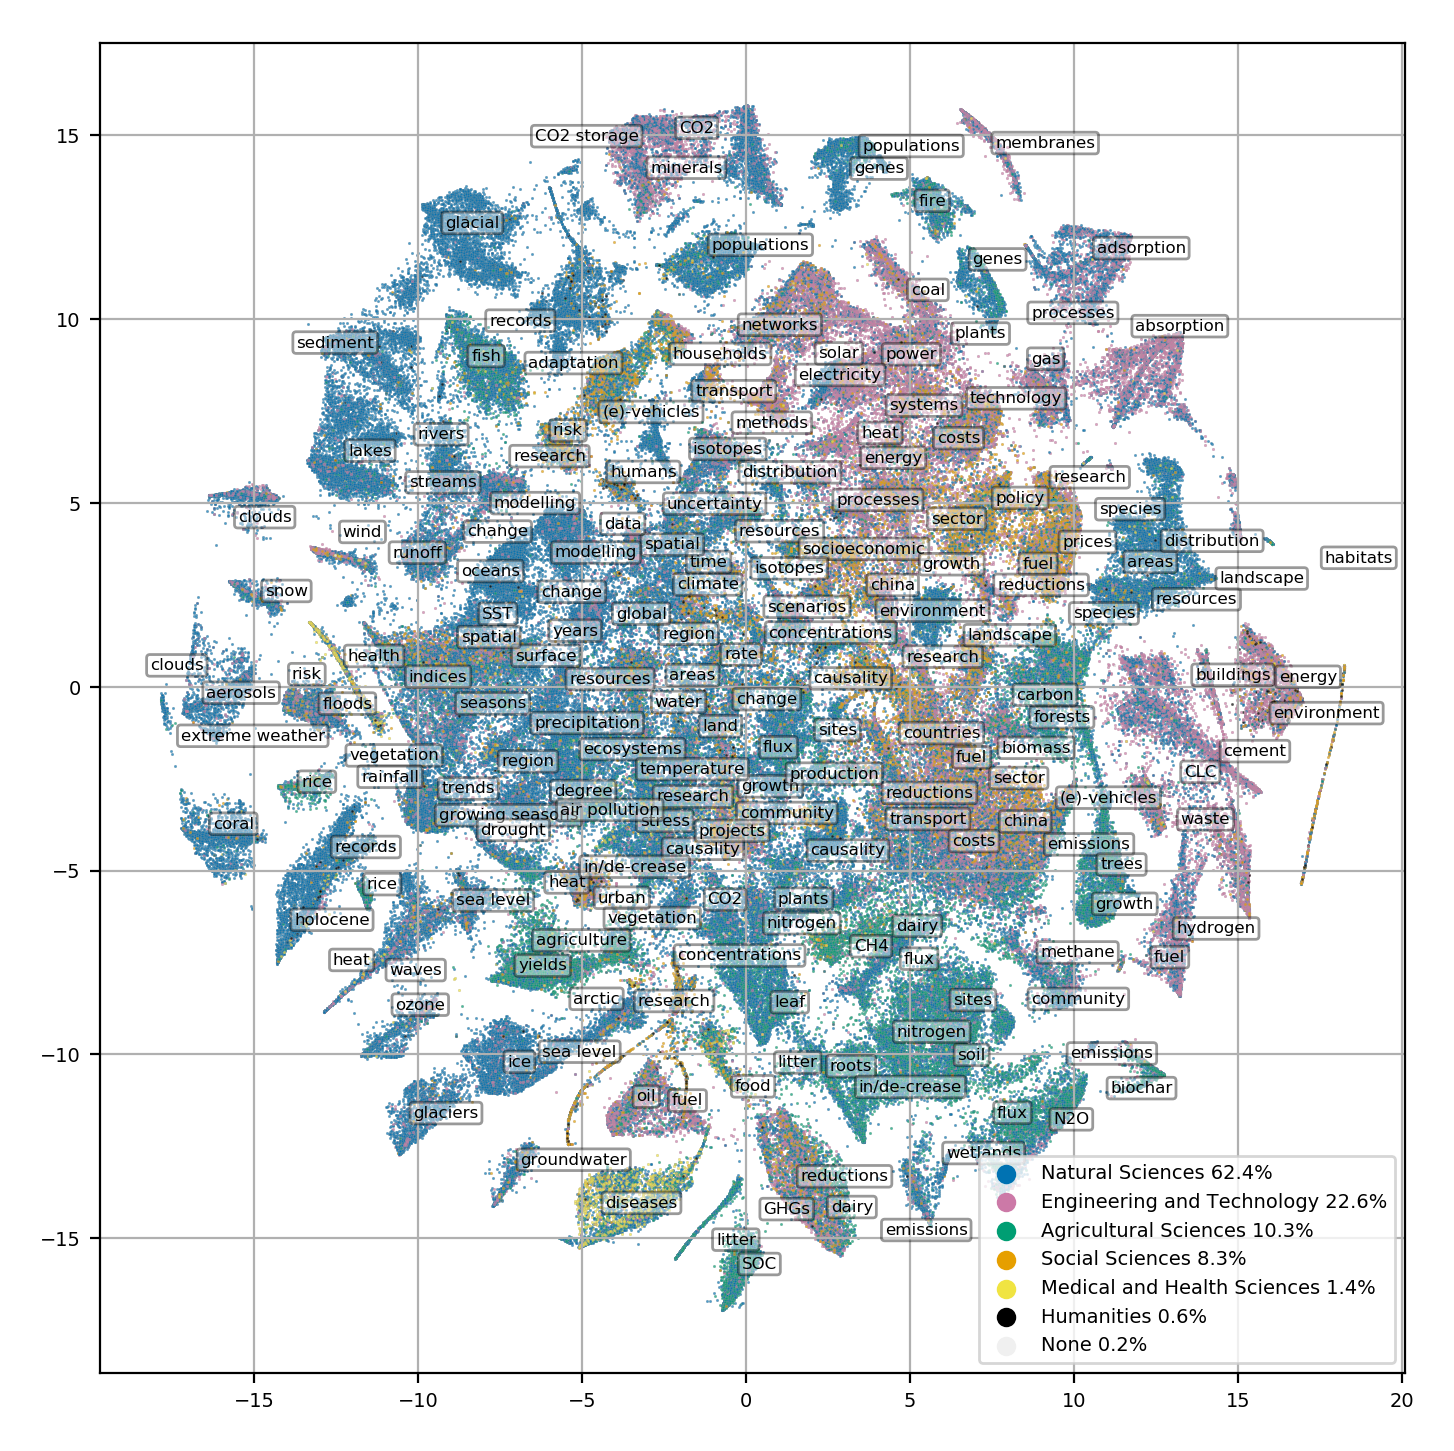
\includegraphics[width=180mm]{tsne_results/plots/run_1861_s_0_p100_all_topic_words_oecds.png}
		\caption{A map of the literature on climate change. Document positions are obtained by reducing the topic scores to two dimensions via t-SNE Documents are coloured by web of science discipline category. Topic labels are placed in the center of each of the large clusters of documents associated with each topic. }
		\label{oecd_topic_map}
	\end{center}
\end{figure}

\subsection*{Social Sciences in IPCC citations}

It was argued after the fifth assessment report that the IPCC needs to do more to incorporate knowledge from the social sciences \cite{Victor2015}, and a scientometric study of the  the third assessment report claimed the IPCC gave a greater \textit{emphasis} to natural sciences and, within the social sciences, to economics. The study, however, operationalised disciplinary emphasis as simply the number of citations from each field. Here we look at \textit{representativeness}, that is, the share of IPCC citations in each field divided by the share of all climate related documents in that field.

\begin{figure}
	\begin{center}
		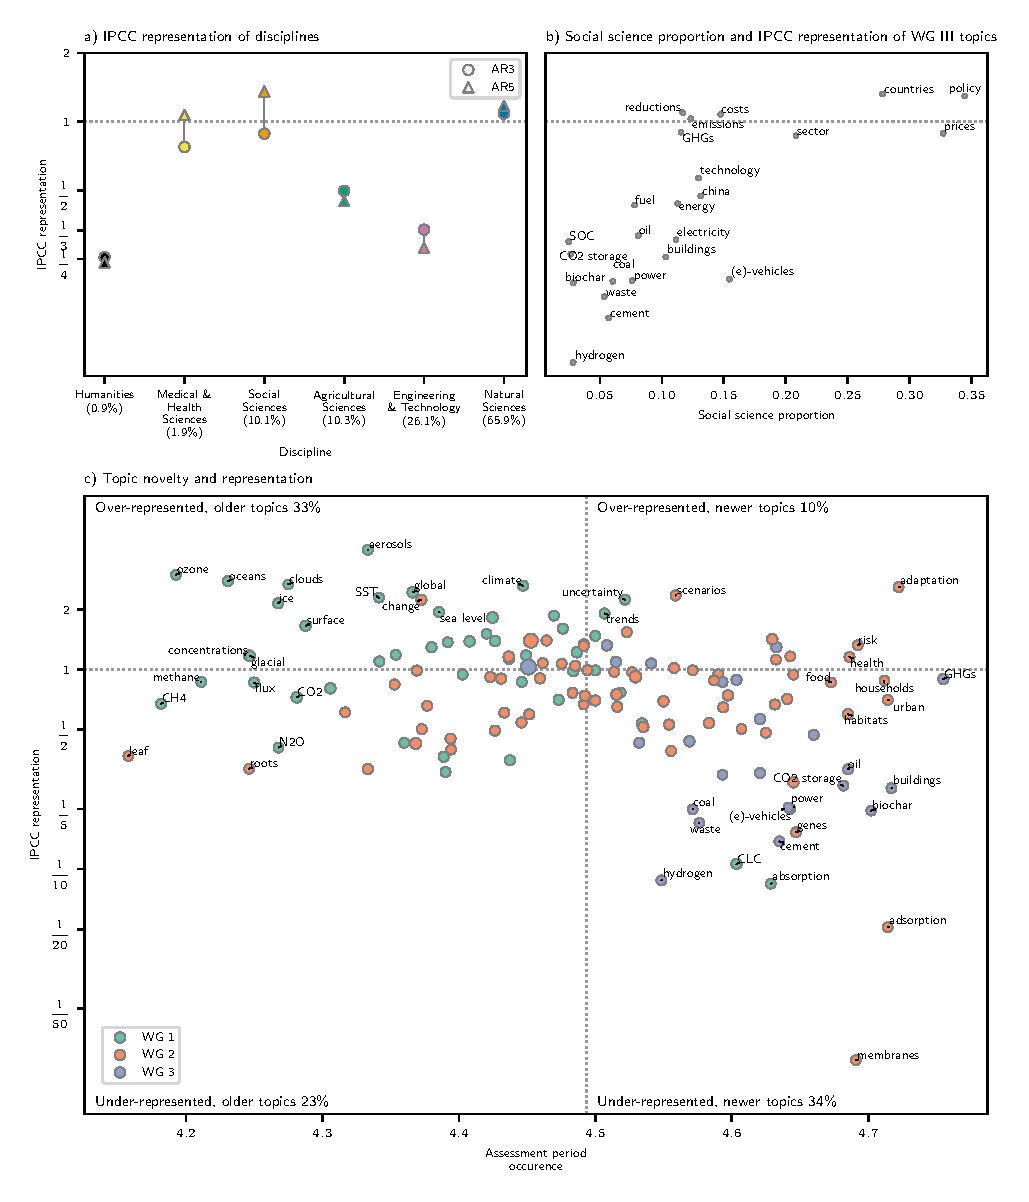
\includegraphics[width=180mm]{plots_pub/big_panel_representation.pdf}
		\caption{\textbf{a)} the representation of each discipline in IPCC reports, \textbf{b)} the representation and social science proportion of WG 3 topics, \textbf{c)} The representation and novelty of all topics }
		\label{oecd_rep}
	\end{center}
\end{figure}


Looked at this way, we see that the social sciences were indeed under-represented in earlier assessment reports, but by the fifth assessment report were over-represented. Although economics was previously over-represented among social sciences, while others were under-represented, more subdisciplines of the social sciences are now over-represented.


\begin{figure}
	\begin{center}
		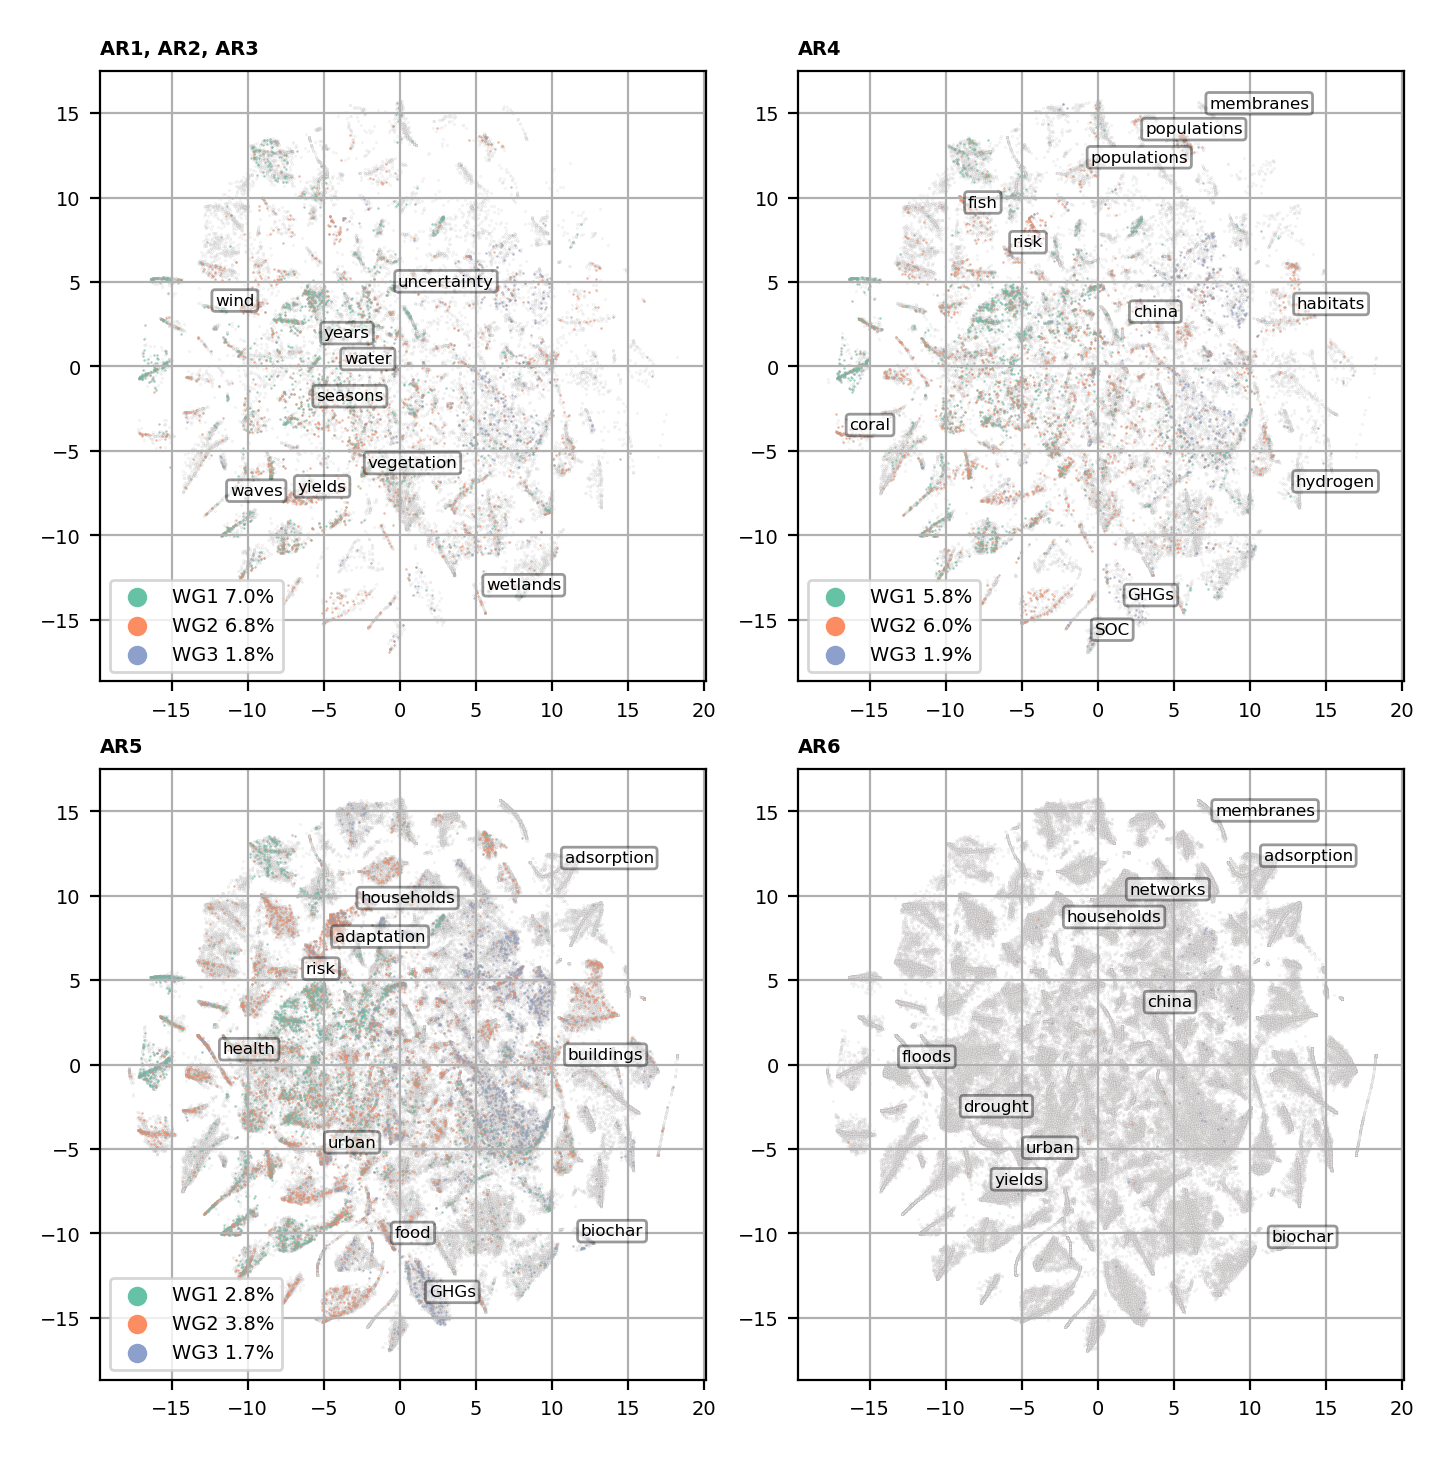
\includegraphics[width=180mm]{tsne_results/plots/run_1861_s_0_p100_evolution_4.png}
		\caption{Evolution of the landscape of climate change literature}
		\label{oecd_topic_map}
	\end{center}
\end{figure}



%\begin{multicols}{2}

%\multicollinenumbers
%\bigskip
%\noindent\textbf{To deal with the wicked problem of climate change, international policy-makers need the IPCC. The IPCC as map-makers.}
%
%The IPCC sees its role as to ``assess on a comprehensive, objective, open and transparent basis the scientific, technical and socio-economic information relevant to [...] climate change'' \citep{IPCC2013}. Climate science is so broad, multi-disciplinary, and laden with uncertainties and values, that the role of the IPCC as assessment maker is vitally important to developing evidence-based international climate policy. In the Pragmatic Enlightened Model of the science-policy interface, the task of assessment making is a cartographic one \citep{Edenhofer2015}. Assessment makers map out the problem and the option space for policy-makers.
%
%
%
%%\bigskip
%%\noindent\textbf{The task of the IPCC has become much more difficult with big literature}
%
%Further, it has been pointed out that, in the age of ``big literature'', providing assessments that are comprehensive, objective and transparent has become much more difficult \citep{Minx2017l}. When the IPCC's citations constitute an ever-decreasing proportion of the totality of science on climate change, questions about the map that the IPCC reports produce become more pressing:
%
%\begin{itemize}
%	\item Is the map up to date?
%	\item Is the map complete?
%	\item Is the map's projection representative? Does it emphasise or obscure certain areas?
%\end{itemize}
%
%
%\section*{The IPCC as an object of scientific investigation}
%
%%%%%%
%
%%\bigskip
%%\noindent\textbf{The IPCC, its reports and processes have been the object of study before. These are also hampered by problems of scale though}
%
%Various researchers have attempted to do empirical research on the assessment reports, and processes of inter. alia. the IPCC \citep{jabbour2017, Bjurström2011, Corbera2016, Hulme2016}. Among the clear conclusions is that policy makers, when asked about their interactions with the IPCC call for a greater focus on solutions \citep{Kowarsch2017}. Studies that look directly at the content of IPCC reports, though, are similarly challenged by the the size of the literature that the reports assess. Without engaging with this literature, the conclusions drawn lack a reference point, and the phenomena identified (such as an over-representation of the natural sciences in IPCC citations \cite{Bjurström2011}) are hard to disentangle as specific to the way the IPCC assesses its literature, rather than a feature of the literature itself. 
%
%%\bigskip
%%\noindent\textbf{Some literature exists on bibliometrics and climate change, but tends not to deal with text}
%
%Some studies have attempted to identify and characterise the literature on climate change through bibliometric techniques \citep{Haunschild2016, Grieneisen2011}. Such studies are the jumping off point for this work, and form the basis of the identification strategy for the literature, but they do not engage with the \textit{texts} of the work identified, nor do they make the link to the IPCC. A growing body of scientific work deals with the unsupervised analysis of texts using topic modelling \cite{Lee1999,Blei2003, Greene2016, Roberts2013}. Applications to the field of climate change though are rare and often limited to closer analysis within sub-topics \cite{Grubert2017}, or calls for their greater use \cite{Grubert2016}. 
%
%\section*{A problem of scale}
%
%
%%\bigskip
%%\noindent\textbf{The scale of the problem in context}
%
%\begin{table}
%	\scriptsize
%	\begin{tabular}{|l |p{1.8cm} p{1.8cm} p{1.8cm} p{1.8cm} p{1.8cm} p{1.8cm}|} 
\hline 
&\textbf{AR1} & \textbf{AR2} & \textbf{AR3} & \textbf{AR4} & \textbf{AR5} & \textbf{AR6}\\ \hline\textbf{Years} &1986-1989 & 1990-1994 & 1995-2000 & 2001-2006 & 2007-2013 & 2014-\\ 
\textbf{Documents} &1,167 & 8,539 & 21,716 & 38,750 & 134,413 & 201,606\\ 
\textbf{Unique words} &2,000 & 12,480 & 23,346 & 34,637 & 71,867 & 94,746\\ 
\textbf{New words} & change (560) & oil (287) & downscaling (217) & sres (234) & biochar (1,791) & mmms (313)\\ & climate (428) & deltac (283) & degreesc (187) & petm (95) & redd (1,113) & cop21 (234)\\ & co2 (318) & whole (256) & ncep (130) & amf (88) & cmip5 (679) & c3n4 (214)\\ & climatic (289) & tax (254) & fco (107) & sf5cf3 (86) & cmip3 (587) & sdg (187)\\ & model (288) & landscape (249) & pfc (98) & clc (81) & mofs (299) & zika (182)\\ & atmospheric (281) & alternative (243) & otcs (98) & embankment (81) & sdm (297) & ndcs (168)\\ & effect (280) & availability (242) & dtr (95) & cwd (79) & mof (275) & indc (164)\\ & global (224) & life (239) & nee (89) & etm (75) & biochars (252) & indcs (134) \\ \hline
\end{tabular}

%	\caption{Growth in climate change literature}
%	\label{growthtable}
%\end{table}
%
%The case for a greater application of text-mining approaches in understanding and assisting the IPCC is made by the scale of the challenge it faces, depicted in table \ref{growthtable}. Less than a thousand documents relevant to climate change were published before the first assessment report (see Methods for data, exclusions and processing). The abstracts of these documents contained 1,380 unique terms. In the three complete years since the publication of AR5, 128,266 documents have been published, containing 74,196 unique terms. The new words in each assessment period unearthed by a basic machine-reading of the literature already give an indication of the how the field has expanded. They chart the emergence of
%
%\linespread{1}
%\begin{itemize}
%	\item new compounds or materials, such as trifluoromethyl sulfur pentafluoride (SF5CF3) in AR4, or mixed matrix membranes (MMMs) in AR6
%	\item new models, or modelling approaches, such as HadCM2 in AR3, or CMIP in AR5 and AR6.
%	\item the involvement of new actors, such as NCEP (National Centers for Environmental Prediction) in AR3
%	\item new approaches, such as biochar and REDD in AR5
%	\item new applications of equipment, such as OTCs (Open-top Chambers) in AR3;
%	\item new phenomena in relation to climate change, such as zika and twitter;
%	\item and new concepts, such as CO2 fugacity (fco) in AR3
%\end{itemize}
%\linespread{1.5}
%
%
%
%
%%To put this into context, the 1,189 chapters of the Bible contain a vocabulary of 11,977 unique words. Put another way, 
%To put this growth into context, the 236,634 publications published in AR5 and AR6 are significantly larger than the 178,118 publications recorded in the first volume of the `Catalogue of Scientific Papers', compiled by the Royal Society to record the entirety of scientific output from 1800 to 1863 \citep{Csiszar2017}. In the last 10 years, climate science has produced significantly more papers than the were published across all scientific disciplines in the first half of the 19th Century.
%
%
%
%
%%\begin{figure}
%%	\begin{center}
%%		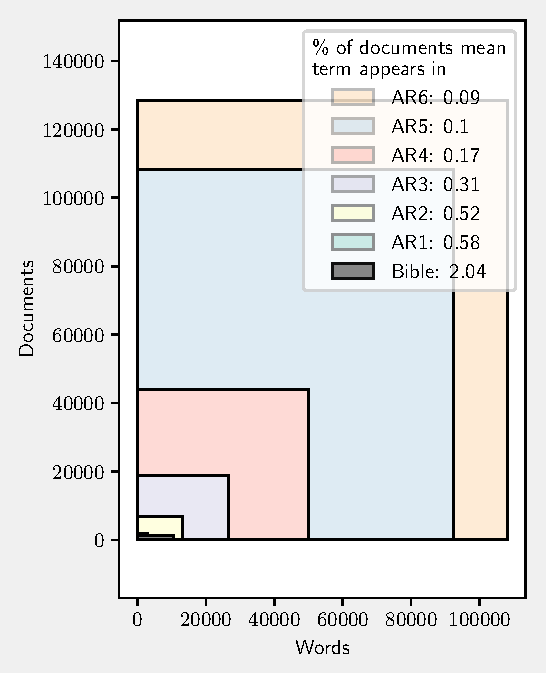
\includegraphics[width=0.5\linewidth]{plots/literature_size/volume_variety.pdf}
%%		%\captionof{figure}
%%		\caption{The volume and variety of literature on climate change has grown to unmanageable proportions. Each box represents a document-term matrix (unique documents x unique terms) of the abstracts written in each assessment period. The percentage of documents in which the average word occurs in is given in the key.
%%		}
%%		\label{growth}
%%	\end{center}
%%\end{figure}
%
%
%%\bigskip
%%\noindent\textbf{Machine reading to deal with scale problems in the making and assessing of maps}
%
%
%Clearly, if the IPCC is to continue producing comprehensive assessments, it has to engage in machine-reading in order to remain anchored to the wider literature. Without such an approach, it becomes harder to justify which ever-diminishing proportion of the wider literature is included in assessments. The same arguement holds for scholars and critics of the IPCC. Without machine reading the literature at large, it becomes harder to analyse or criticise, with quantitatively evidenced claims, the outcomes of assessment processes.
%
%
%%\bigskip
%%\noindent\textbf{Dimension reduction makes possible the description in reduced form, and with less human bias, of unmanageably large datasets}
%
%%\citep{Greene2016} \citep{Lee1999}
%In order to draw substantive messages from this high-dimensional document-word space, we apply a form of dimensionality reduction called topic-modelling \citep{Blei2010}. The non-negative matrix factorisation (NMF) approach to topic modelling is based on generating a ``perception of the whole based on perception of its parts'' \citep{Lee1999}. Here the corpus of documents (whole) is summarised by its parts (topics), which appear in varying proportions in each of the documents. Importantly, in such approaches, the parts are not pre-defined, but learned by the algorithm, leveraging systematic co-occurences of words within documents. This makes the discovery of unlooked-for features possible and can reduce the human bias risked by the pre-definition of categories. 
%
%%\bigskip
%%\noindent\textbf{Machine reading is a supplement to assessment-making and not free from bias; a topography is not a map}
%
%Despite these advantages, machine reading and machine learning approaches can of course not replace the task of human assessment-making. The contribution that could be made, though, is to pre-process the literature, producing a topographical map, used to navigate the literature while producing a more detailed assessment with human judgement. In fact this happens already - when IPCC authors search for literature on a topic, the results which appear on the search engine they use will be subject to algorithms based on the processing of millions of records of article text and metadata. This can be done in a much more systematic way when scientists perform directed analyses of the literature at scale. 
%
%
%%\bigskip
%%\noindent\textbf{This study's contribution. Overarching themes, structure of the literature, development, relation to IPCC}
%
%In applying a dynamic version of NMF \cite{Greene2016}, this study demonstrates how topic modelling can be used to gain an overview of an otherwise unmanageably large body of literature. This overview, or topography, describes the thematic development of the climate change literature and, in a novelly systematic way, examines how comprehensively the IPCC has been able to engage with it. In pulling together strands from text-mining, bibliometrics, and the study of science and policy, this study advances our understanding of the literature on climate change and the role of the IPCC in communicating this to policy makers.
%
%
%\section*{Results}
%
%Table \ref{top-topics} shows the 10 most prominent topics within the literature on climate change. The topics are characterised by the (stemmed) words that define them, and by the documents which are most well described by them. For example, the topic ``energi, renew, consumpt'' features the words energi, renew, consumpt,
%effici, demand,
%save, sector, sourc,
%industri, use, and best describes the documents ``Energy issues and energy priorities'' \cite{Demirbas2008} and ``Energy efficiency and CO2 emissions in Swedish manufacturing industries'' \cite{PardoMartinez2013}. The topics learned by dynamic NMF identify a set of interpretable topics and can identify which documents belong to these topics. 
%
%\begin{table}
%	\scriptsize
%	\begin{tabular}{p{1.9cm} p{3cm} p{7.5cm} r}
\toprule
                      title &                                                                            top words &                                                                                                                                                                                                                                                                top docs &   share \\
\midrule
      climat, chang, impact &          [climat, chang, impact, respons, futur, effect, shift, sensit, affect, may] &                                                                                                                                                  \parbox[t]{7.5cm}{Climate oscillations and changes over Russia; \\World Regionalization of Climate Change (1961-2010)} &  2.73\% \\
     soil, moistur, microbi &       [soil, moistur, microbi, organ, respir, content, miner, depth, matter, efflux] &                                                                                    \parbox[t]{7.5cm}{PARTITIONING OF SOIL RESPIRATION IN A FIRST ROTATION BEECH PLANTATION; \\Responses of soil respiration to N fertilization in a loamy soil under maize cultivation} &  2.73\% \\
       emiss, reduct, reduc &      [emiss, reduct, reduc, greenhous, factor, total, estim, inventori, nox, measur] &                                                                                                             \parbox[t]{7.5cm}{China's CH4 and CO2 emissions: Bottom-up estimation and comparative analysis; \\Monitoring total emissions from industrial installations} &  2.21\% \\
   carbon, dioxid, sequestr &   [carbon, dioxid, sequestr, sink, organ, cycl, storag, stock, terrestri, atmospher] &                             \parbox[t]{7.5cm}{Interpreting carbon-isotope excursions: carbonates and organic matter; \\PARTICULATE FLUXES OF CARBONATE AND ORGANIC-CARBON IN THE OCEAN - IS THE MARINE BIOLOGICAL-ACTIVITY WORKING AS A SINK OF THE ATMOSPHERIC CARBON} &  1.74\% \\
      temperatur, air, mean &  [temperatur, air, mean, surfac, minimum, maximum, daili, increas, effect, degreesc] &                                                                                                     \parbox[t]{7.5cm}{Observed changes in shallow soil temperatures in Northeast China, 1960-2007; \\Beyond the Mean: Biological Impacts of Cryptic Temperature Change} &  1.71\% \\
      record, dure, glacial &       [record, dure, glacial, reconstruct, last, period, holocen, event, late, core] &                                                           \parbox[t]{7.5cm}{HIGH-RESOLUTION CLIMATE RECORDS FROM THE NORTH-ATLANTIC DURING THE LAST INTERGLACIAL; \\HIGH-RESOLUTION CLIMATIC INFORMATION FROM SHORT FIRN CORES, WESTERN DRONNING MAUD LAND, ANTARCTICA} &   1.7\% \\
     speci, distribut, rang &          [speci, distribut, rang, rich, invas, nich, predict, extinct, shift, abund] &                               \parbox[t]{7.5cm}{Northward range extensions of some mesopelagic fishes in the Northeastern Atlantic; \\Natural occurrence and backwater infection of C-4 plants in the vegetation of the Yangtze hydropower Three Gorges Project region} &   1.7\% \\
 increas, concentr, decreas &   [increas, concentr, decreas, effect, atmospher, doc, result, organ, nutrient, may] &                                                          \parbox[t]{7.5cm}{TERRESTRIAL HIGHER-PLANT RESPONSE TO INCREASING ATMOSPHERIC [CO2] IN RELATION TO THE GLOBAL CARBON-CYCLE; \\Hydrological response to climate change in the Black Hills of South Dakota, USA} &  1.61\% \\
      forest, tropic, stand &       [forest, tropic, stand, deforest, disturb, stock, boreal, redd, harvest, wood] &  \parbox[t]{7.5cm}{Spatially explicit estimates and temporal changes of forest tree biomass in a typical department of forest management, Turkey; \\Analysis of the changes in forest ecosystem functions, structure and composition in the Black Sea region of Turkey} &  1.56\% \\
    energi, renew, consumpt &        [energi, renew, consumpt, effici, demand, save, sector, sourc, industri, use] &                                                                                                                                       \parbox[t]{7.5cm}{Energy issues and energy priorities; \\Energy efficiency and CO2 emissions in Swedish manufacturing industries} &  1.56\% \\
\bottomrule
\end{tabular}

%	\caption{Top 10 topics in climate change literature}
%	\label{top-topics}
%\end{table}
%
%Such first results show the promise of topic modelling in the identification of studies in a thematic area, which is of high value to assessment exercises like the IPCC, but in themselves do not give a sense of the broad structure of the corpus. Figure \ref{map-double} projects the documents on to a two dimensional representation of the their topic composition derived through t-distributed Stochastic Network Embedding (t-SNE) \cite{vandermaaten2008}. In this approach, documents are positioned close to other documents with similar topic compositions. This projection enables us to show a topography of the whole literature on climate change.
%
%\begin{figure}
%	\begin{center}
%		%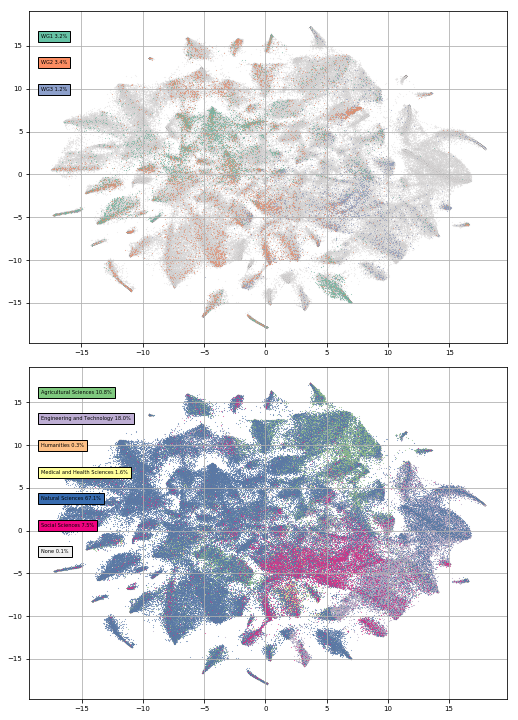
\includegraphics[width=1\linewidth]{tsne_results/plots/run_665_s_0_p200_double.pdf}
%		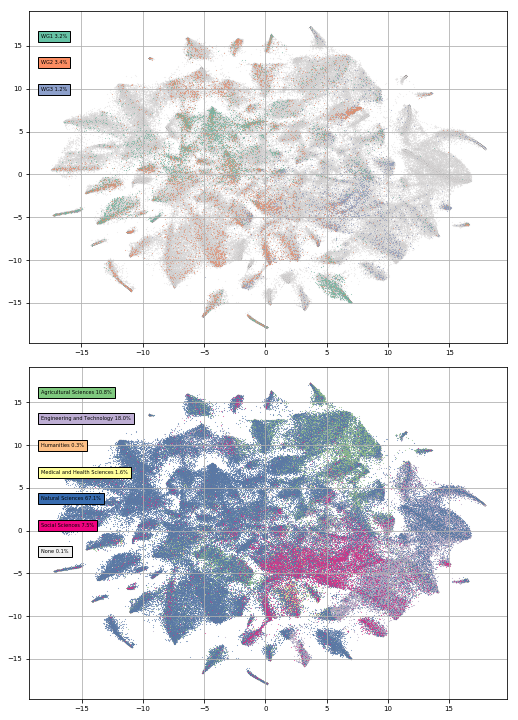
\includegraphics[width=0.85\linewidth]{tsne_results/plots/run_665_s_0_p200_double.png}
%		\caption{A map of the literature on climate change. Document positions are obtained by reducing the topic scores to two dimensions via t-SNE Documents are coloured by working group citations (top) and web of science discipline category (bottom). See SI table for topic composition of each grid square}
%		\label{map-double}
%	\end{center}
%\end{figure}
%
%
%In the two panels of the figure, the documents are coloured by the IPCC working group which cites them (if any), and the disciplinary classification according to the Web of Science. The topic structure cuts across working group and disciplinary lines, but the disciplinary and working group structure is clearly visible in the topography. For example, in the south-eastern section of the map, we can see a concentration of documents in the social sciences that were cited by working group III (mitigation).
%
%The topography\_map\_reference.csv [ \url{https://github.com/mcallaghan/cc-topography/blob/master/tables/tsne_topic_index_665.csv}] file in the supporting materials aids more detailed analysis of the map, describing the topic composition of each square. For example the square whose center is [12.5,-7.5] is made up of the topics \{energi, renew, consumpt\}, \{fuel, fossil, engin\}, \{emiss, reduct, reduc\}, \{countri, develop, trade\} and \{cost, optim, price\}, typical social science, working group III topics. The square whose center is [-17.5,-2.5], containing mostly working group I (the physical science basis) documents on the other hand, is made of largely by the topic {ozon, stratospher, tropospher} as well as by {increas, concentr, decreas}, and {climat, chang, impact}.
%
%%\bigskip
%%\noindent\textbf{A topographical map of climate change documents shows the broad structure of climate change literature}
%Figure \ref{map-growth} shows the evolution of the landscape of climate change literature over the 6 (including the in progress AR6) assessment periods of the IPCC. In each assessment period, the grid squares which contain a higher (lower) proportion of documents than in the previous assessment period are coloured green (red). This mapping allows us to identify topic areas as they appear in the literature. For example, the square with the center [-12.5,12.5] is composed largely of the topic \{coral, reef, bleach\}, and contained no documents before a sudden growth in AR3. Indeed, the topic of coral bleaching  was little discussed in the context of climate change before AR3, with just two out of 693 results from Web of Science for the terms  "Coral bleaching" AND "climate change" published before 1996. More recently, the square [12.5,12.5] identifies the topic \{biochar, amend, applic\} as a quickly emerging field within climate change in present times.
%
%\begin{figure}
%	\begin{center}
%		%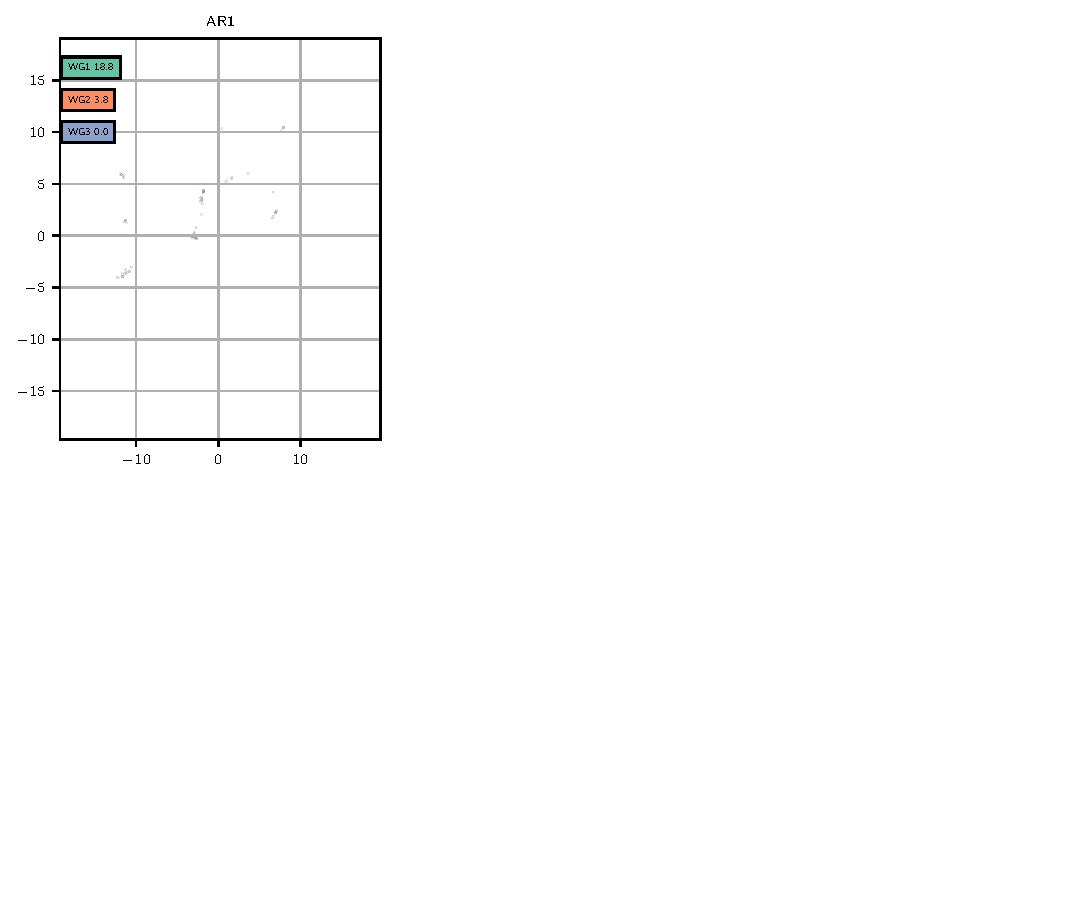
\includegraphics[width=1\linewidth]{tsne_results/plots/run_665_s_0_p200_evolution.pdf}
%		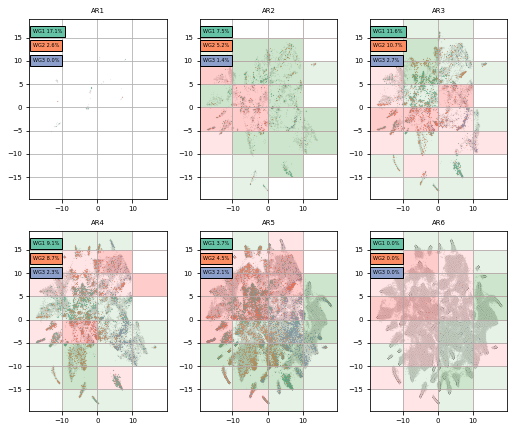
\includegraphics[width=1\linewidth]{tsne_results/plots/run_665_s_0_p200_evolution.png}
%		\caption{The evolution of the landscape of climate change literature}
%		\label{map-growth}
%	\end{center}
%\end{figure}
%
%
%%\begin{figure}
%%	\begin{center}
%%		%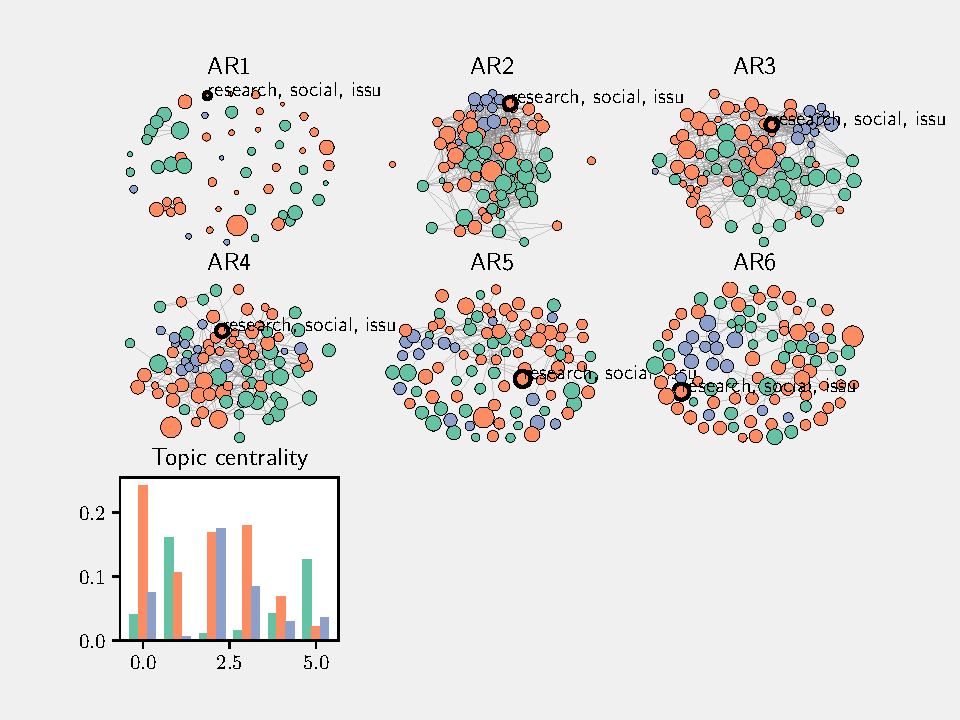
\includegraphics[width=1\linewidth]{plots/network_development_wgs_665.pdf}
%%		\caption{The development of the topic-document correlation network over IPCC assessment periods.}
%%		\label{}
%%	\end{center}
%%\end{figure}
%
%%\bigskip
%%\noindent\textbf{The topic-document correlation network is densest in AR2 and 3 but becomes more fragmented over time}
%%
%%(partly: Model less good at describing literature later on)
%
%%\bigskip
%%\noindent\textbf{Working groups are clustered together [dynamics], with topics like [x] containing documents across working groups and topics like [y] important network nodes}
%
%The dynamic nature of the topic model also allows us to identify changes within topics. SI figure \ref{sus} shows the evolution of the topic \{research, social, issu\}. In this overarching topic on research priorities we can detect an increasing prominence of the word ``sustainability''.
%
%Finally, by comparing the topic distribution across all documents (published before the end of AR5) with the topic distribution across documents that were cited by the IPCC, we can identify those topics which were over- or under- represented, with respect to the underlying literature, in IPCC reports. Figure \ref{representation} plots the representation and novelty of all topics in the model, labelling those topics most under- or over-represented. The topics are coloured according to the working group from which most IPCC citations to its documents came.
%
%The negative slope of the plot shows that the IPCC better represents those topics which have a longer history in the literature. The majority of well represented older topics come from working group I, such as \{aerosol, cloud, radiat\}. New topics in working group II on adaptation and vulnerability are well represented in IPCC reports. However, a cluster of new topics on mitigation issues appear to be under-represented by the IPCC. Moreover, these topics, such as those on buildings, waste, biochar, carbon capture and carbon storage are those that deal with climate solutions.
%
%
%\begin{figure}
%	\begin{center}
%		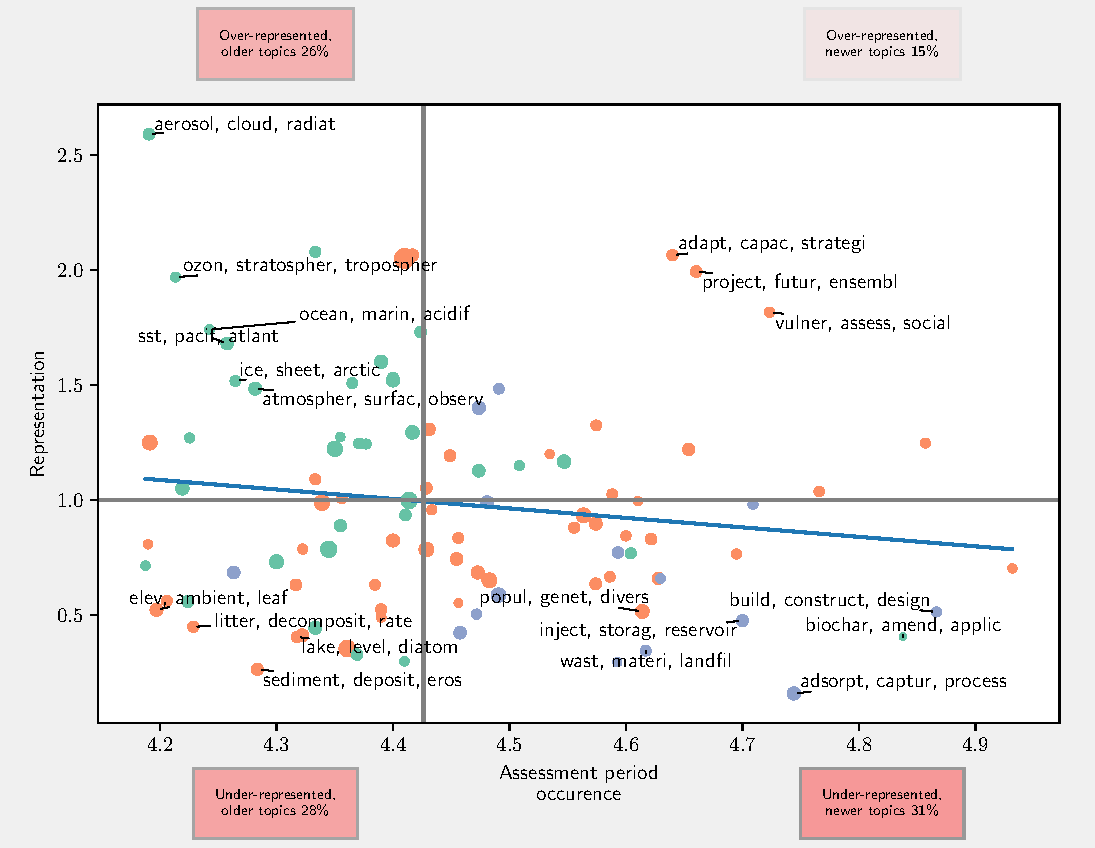
\includegraphics[width=1\linewidth]{plots/ipcc_representation/ipcc_rep_new665_all.pdf}
%		\caption{Representation and newness of dynamic topics}
%		\label{representation}
%	\end{center}
%\end{figure}
%
%
%%\bigskip
%%\noindent\textbf{Sustainability has been an increasingly important theme in an overarching topic about environmental sciences}
%%
%%(compare to biochar, which is much more recent)
%
%
%
%
%\section*{Discussion}
%
%%\bigskip
%%\noindent\textbf{Solutions, policies and science}
%%
%%What do policy-makers mean when they ask for more solutions
%
%The results from a dynamic topic model of climate change literature delineate the structure and evolution of the field, telling its history and identifying areas of rapid growth that are of high relevance for future assessments. Further, they suggest that the demand by policy-makers from the IPCC for a greater focus on solutions is well-founded. Topics related to climate solutions are the least well represented in the IPCC's assessments.
%
%%\bigskip
%%\noindent\textbf{Perfect representation is not necessarily desirable, but the skewedness should be known}
%There may well be excellent reasons for over- or under-representation of topics in IPCC reports, and indeed it is the institution of the IPCC, not machines, who can best make judgements about what to include and what not to include. However, it is unclear whether the decisions which resulted in such unequal distributions were made consciously, on the basis of an understanding of the breadth of the extant literature. For future assessments to be relevant, transparent and comprehensive in the age of big literature, these decisions should be supported by machine-supported engagement with the literature as a whole.
%
%
%%Increase in the frequency of the use of the term ``solutions'' \citep{jabbour2017},
%
%%\section*{Methods}
%%\label{methods}
%%
%%
%%
%%\subsection*{Data}
%%This study reproduces the query developed by \citep{Grieneisen2011}, which is carried out on Web of Science. Though not exhaustive, it gives a good coverage of
%
%\pagebreak
%
%
%\documentclass{article}
\usepackage[a4paper, total={6in, 8in}]{geometry}
\usepackage{graphicx}
\usepackage{url}
\usepackage{natbib}
\usepackage{todonotes}
\usepackage{booktabs}
\usepackage{lineno}
\usepackage{color}
%\usepackage{auto-pst-pdf}
\usepackage[colaction]{multicol}
\usepackage{caption}
\usepackage{svg}
\usepackage{authblk}
\usepackage{standalone}
\usepackage[section]{placeins}

\makeatletter
\renewcommand{\maketitle}{\bgroup\setlength{\parindent}{0pt}
	\begin{flushleft}
		
		{\huge\textbf{\@title}}
		
		\bigskip
		
		{\large\textbf{\@author}}
		
		\bigskip
		
		{\large{Draft current \@date}}
		
	\end{flushleft}\egroup
}
\makeatother


\begin{document}
	% Title
	\title{A Topic Model of Climate Change Literature}
	\title{Words, words, words: Mapping the Matter of Climate Change Literature}
	\title{A Topography of Climate Change Research - Methods}
	\author[1,2]{Max Callaghan}
	
	\affil[1]{Mercator Research Institute on Global Commons and Climate Change, Torgauer Straße, 10829 Berlin, Germany}
	\affil[2]{School of Earth and Environment, University of Leeds, Leeds LS2 9JT, United Kingdom}
	\maketitle
	\begin{linenumbers}
	
	\setcounter{figure}{0}
	\renewcommand\thefigure{SI.\arabic{figure}}  
		
	\subsection*{Data}
	
	This study reproduces the query developed by \citep{Grieneisen2011}, which is carried out on the Web of Science core collection. Though not exhaustive, the Web of Science gives a good coverage of the literature in major peer-reviewed journals. The Web of Science data gives us a disciplinary classification (based on the journal) and publication year, among other metadata, for each document.	Each document is assigned to an assessment period according to the timeline shown in table 1.
	
	We use the references scraped from IPCC assessment reports from \citep{Minx2017l}, and attempt to match these with the results from the Web of Science. We use doc2vec similarity scores \cite{Le2014} to identify the 500 most similar titles for each reference, and count the document as a match if the jaccard similarity score of the two word shingles of the reference title and the document title is greater than 0.5 \cite{Khabsa2014}. Table \ref{ipcc-matching} shows the percentage of IPCC citations matched in each working group for each assessment report. This is significantly lower in earlier periods, as data coverage and quality of citation databases is lower for earlier periods. Matching in WG III is also lower, suggesting a greater share of non-peer review literature, or literature not directly mentioning climate change, but related to it's mitigation (for example on energy policy).
	
		\begin{table}[htp]
			\begin{center}
		\begin{tabular}{lrrrrr}
\toprule
AR &  1 &   2 &   3 &   4 &   5 \\
WG &    &     &     &     &     \\
\midrule
1  & 8\% & 25\% & 37\% & 47\% & 58\% \\
2  & 6\% & 12\% & 30\% & 38\% & 47\% \\
3  & 3\% &  9\% & 15\% & 22\% & 35\% \\
\bottomrule
\end{tabular}

	\caption{IPCC matching}
	\label{ipcc-matching}
	\end{center}
\end{table}
	
		
	\subsection*{Pre-processing}
	
	Data quality in earlier Web of Science results is poorer, and some documents have missing abstracts. In the quantification of the size of the literature and its vocabulary in table \ref{tab}, titles are substituted for abstracts where they are not available.  The words of the documents are lemmatized, replacing different forms of the same word (i.e. word/words) with a single instance. Commonly occurring words, or ``stopwords'' are removed, as are all words shorter than 3 characters, and all words containing only punctuation or numbers.
	
	The documents are transformed into a document-term matrix, where each row represents a document, and each column represents a unique word.  Each cell contains the number of that column's terms in that document. Only terms which occur more than once are considered.
	
	For the calculation of the topic model, documents with missing abstracts are ignored, and the document term matrix is transformed into a document
	frequency-inverse document frequency (tf-idf) matrix, where scores are scaled according to the frequency of their occurrence in the corpus. This gives more weight to terms which appear in few documents, and less weight to those which appear in many.
	
	\begin{equation}
	tf(t,d) = f_{t,d} \mathrm{,}\quad idf(t,D) = \log\frac{N}{|\{d \in D:t \in d\}|}
	\end{equation} 
	
	\subsection*{Topic Model}
	
	We use non-negative Matrix Factorisation (NMF) \cite{Lee1999}, an approach to topic modelling which factorises the term-frequency-inverse document frequency matrix \( V \) into the matrices \(W\), the topic-term matrix, and \( H \) the document-topic matrix, whose product approximates \(V\):
	
	\begin{equation}
		V_{i\mu} \approx (WH)_{i\mu} = \sum_{a=1}^{r}W_{ia}H_{a\mu}
	\end{equation}
	
	As demonstrated in Figure \ref{doc-topic}, each topic is represented as a set of word scores, and each document a set of topic scores. The combination of the two give the word scores in the document. For clarity in the figure, these are shown as simple counts, but in the model these are scaled according to each term's frequency within the corpus as explained above.
	
	Topics are calculated using the scikitlearn library \cite{Pedregosa2011}, and are saved in a database and topic visualisation system based on \cite{Chaney2012} \footnote{The system adds new functionality to \cite{Chaney2012} and combines it with a system for managing sets of documents and queries. The code and additional information is published online at \url{https://github.com/mcallaghan/tmv}}. 	
	
	\subsubsection*{Model selection}
	
	Topic models are calculated for 70, 80, 90, 100, 110, 120, 130, 140 and 150 topics. The run with 150 topics was discarded as it contained a topic to which no terms or documents were assigned. The relative usefulness of each model was assessed subjectively by the authors, based on inspection of the online visualisation tool, and the spreadsheet \textbf{topic\_comparison.xlsx} accompanying the supporting information. The spreadsheet shows each set of topics in adjacent columns. Topics from each model are placed next to the topics with the largest number of each topic's 10 highest scoring words in common. This helps authors to find an appropriate level of granularity for the analysis. 
			
	\subsubsection*{Topic Representation and Newness}
	
	To calculate topic representation in IPCC reports we divide each topic's share in the subsample of documents cited by IPCC reports by its share in the whole corpus. 
	
	We calculate a topic's total score as the sum of document-topic scores. A topic's window score is the sum of document-topic scores considering only documents in the given time window. To represent a topic's newness, we multiply each assessment period number by the share of it's total score occurring in that window, and take the mean of these scores. A topic in which 100\% of documents which make it up occurred in assessment period 1 (6) would thereby receive a score of 1 (6), while a topic evenly distributed across all assessment periods would receive a score of 3.5.
	
	
	\subsubsection*{Disciplinary Entropy}
	
	Disciplinary Entropy inverts the measurement of a conference's topical diversity suggested in \cite{Hall2008}, by measuring a topic \(z\)'s entropy \(H\), where 
	
	\begin{equation}
		H(f|z) = -\sum_{i=1}^K \hat{p}(f|z) \log \hat{p}(f|z) 
	\end{equation}
	
	based on the empirical distribution of a field \(f\) in the documents \(d\) in each topic:
	
	\begin{equation}
		\hat{p}(f|z) = \sum_{d:z_d=z} \hat{p} (f|d) \hat{p} (d|z)
	\end{equation}
	
	\subsubsection*{Topic Map}
	The topic model gives us the location of each document in a 140 dimensional topic space, with each dimension corresponding to a that document's \textit{topic-ness} in a given topic. t-Distributed Stochastic Neighbour Embedding (t-SNE) is a dimensionality reduction technique which we use to represent each document's topic scores in 2 dimensions \cite{vandermaaten2008}.

	\begin{figure}
		\begin{center}
			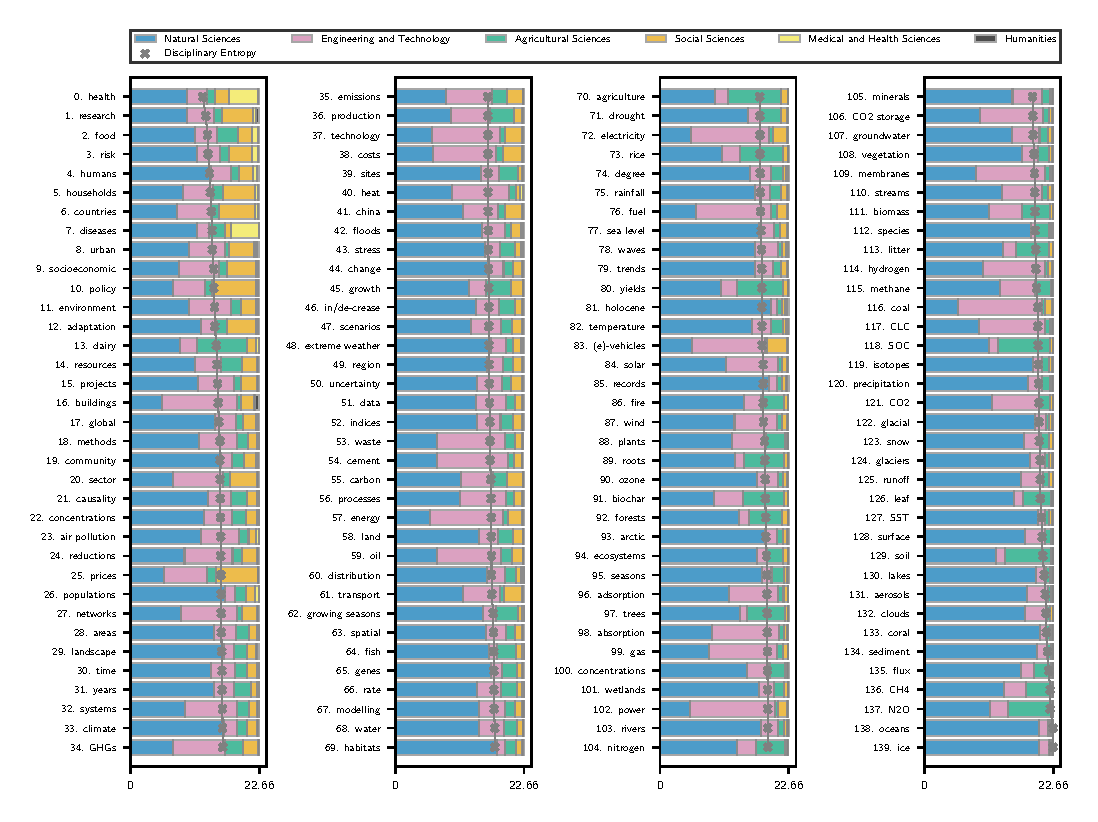
\includegraphics[width=1\linewidth]{plots_pub/topic_oecd_entropy.pdf}
			\caption{SI Disciplinary Entropy}
			\label{dis-entropy}
		\end{center}
	\end{figure}	
	
	
	
	\begin{figure}
		\begin{center}
			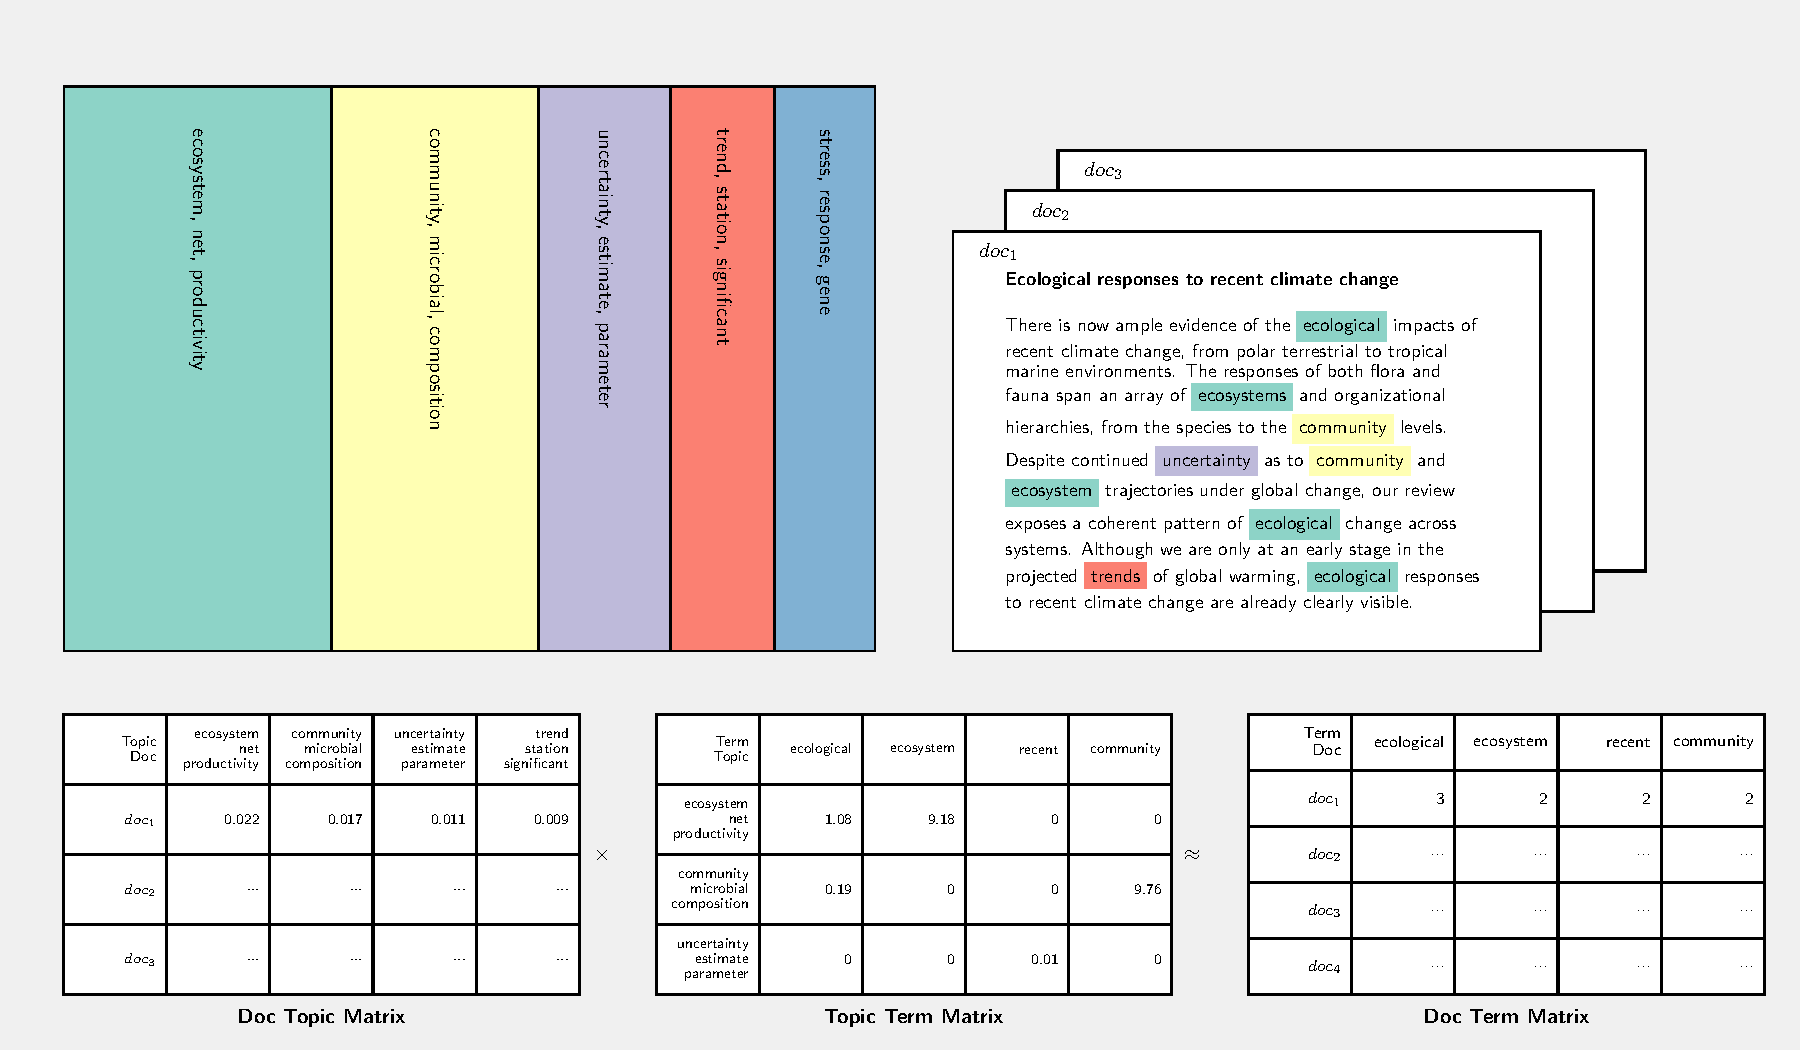
\includegraphics[width=1\linewidth]{plots_pub/single_doc_3_536594_1861.pdf}
			\caption{SI Topic make up of a single document}
			\label{doc-topic}
		\end{center}
	\end{figure}

	\begin{figure}
	\begin{center}
		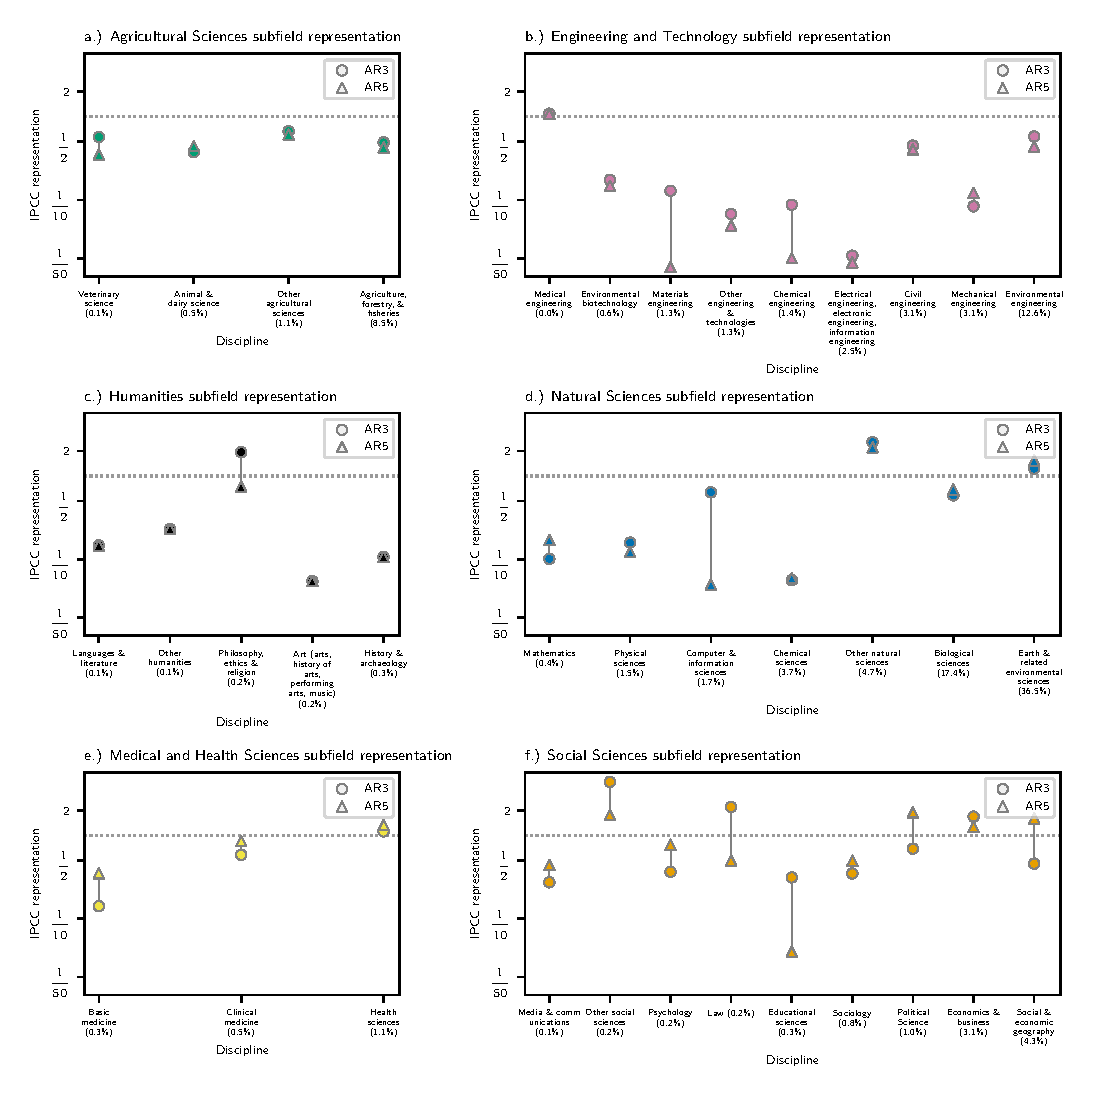
\includegraphics[width=1\linewidth]{plots_pub/ipcc_rep_wcs_simplified.pdf}
		\caption{SI Representation by subfield}
		\label{subfield}
	\end{center}
\end{figure}

\begin{figure}
	\begin{center}
		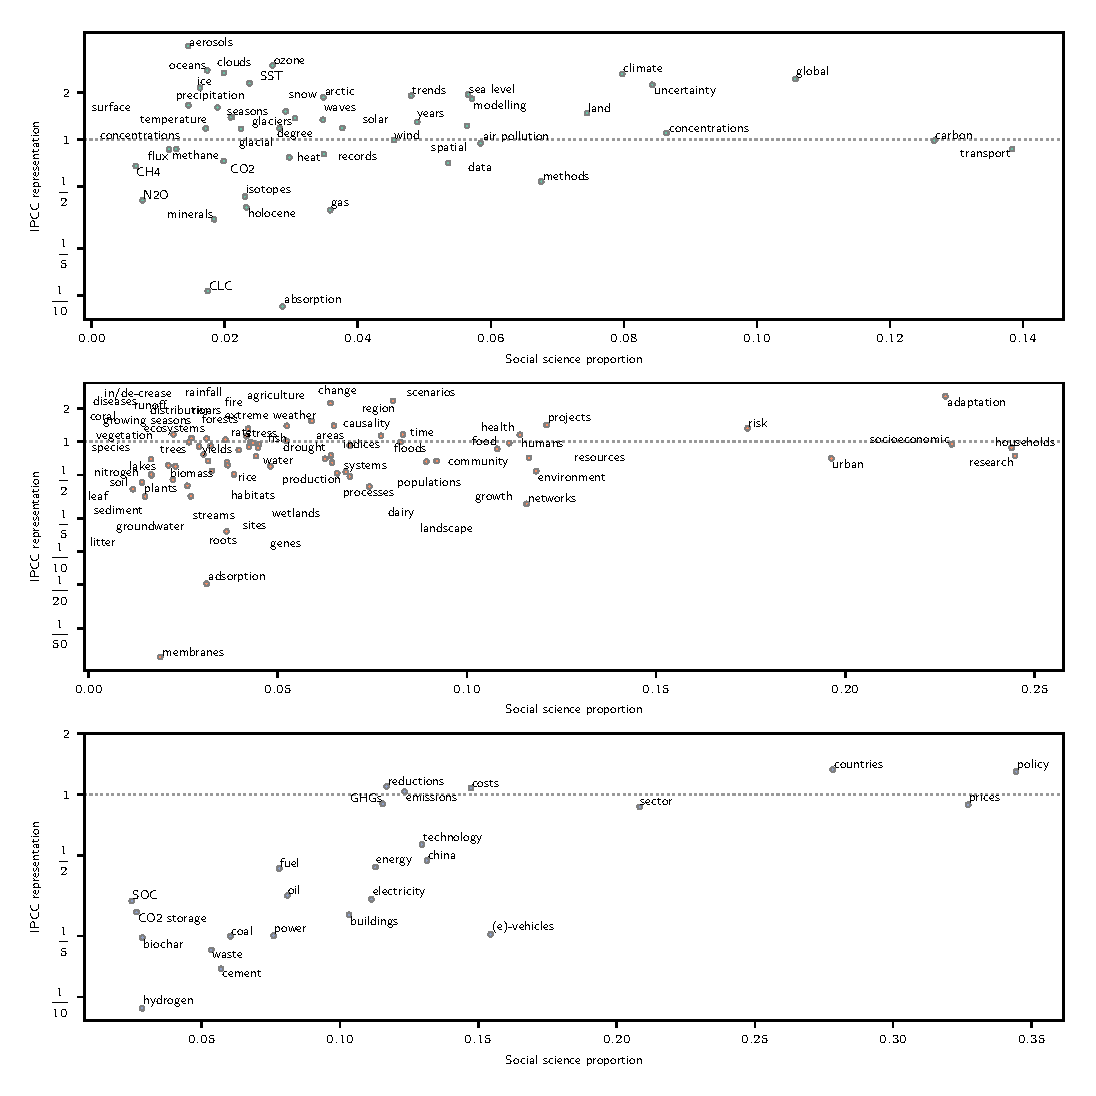
\includegraphics[width=1\linewidth]{plots_pub/wgs_socsci.pdf}
		\caption{SI Social science \& representation in topics across working groups}
		\label{socsci-wgs}
	\end{center}
\end{figure}

\begin{figure}
	\begin{center}
		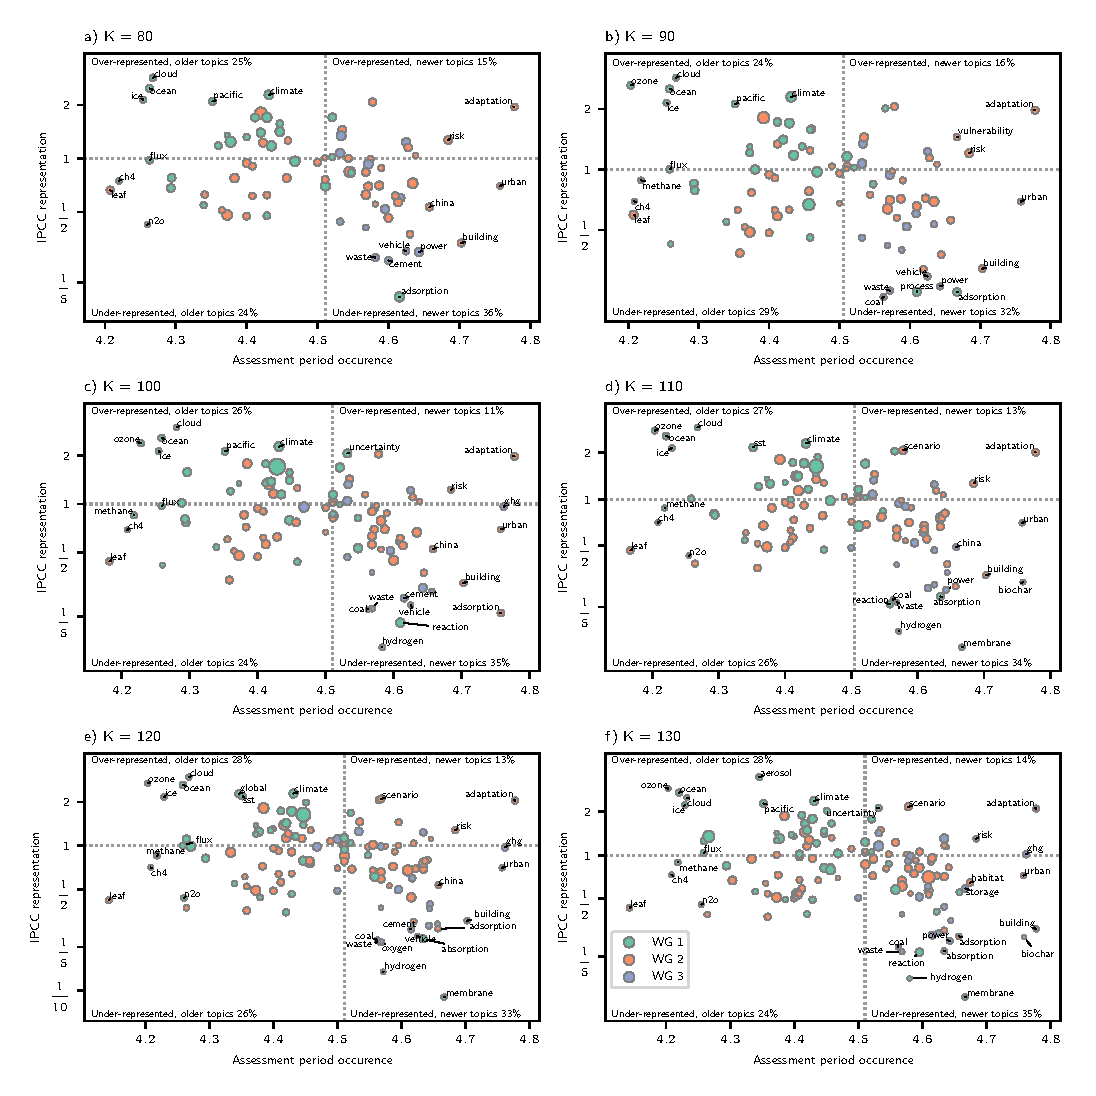
\includegraphics[width=1\linewidth]{plots_pub/topic_rep_ks.pdf}
		\caption{Topic representation over different values of K (number of topics). Topics in the upper or lower 6.66th percentile of either dimension are labelled}
		\label{top-rep-ks}
	\end{center}
\end{figure}

\subsection*{Glossary}


\noindent\textbf{ncep:} National Centers for Environmental Protection

\noindent\textbf{fco:} Fugacity of Carbon Dioxide

\noindent\textbf{pfc:} Perflourocompound

\noindent\textbf{otcs:} Open Top Chambers

\noindent\textbf{dtr:} Diurnal Temperature Range

\noindent\textbf{sres:} Special Report on Emissions Scenarios (200)

\noindent\textbf{petm:} Paleocene Eocene Thermal Maximum

\noindent\textbf{amf:}  Arbuscular Mycorrhizal Fungal

\noindent\textbf{sf5cf3:} trifluoromethyl sulfur pentafluoride (A Potent Greenhouse Gas Identified in the Atmosphere, 2000)

\noindent\textbf{clc:} Chemical Looping Combustion

\noindent\textbf{cwd:} Coarse woody debris

\noindent\textbf{etm:} Enhanced Thematic Mapper (NASA satellite sensor)

\noindent\textbf{cmip5:} Coupled Model Intercomparison Project 5 (Starting 2008)

\noindent\textbf{cmip3:} Coupled Model Intercomparison Project phase 3 (first published 2007 \cite{Meehl2007})

\noindent\textbf{mofs:} metal-organic frameworks (for CO2 storage)

\noindent\textbf{sdm:} statistical-dynamical model

\noindent\textbf{mmms:} Mixed Matrix Membranes (for CO2 capture)

\noindent\textbf{cop21:} 21st Conference of Parties (Paris 2015) 

\noindent\textbf{c3n4:} Carbon nitride (a synthetic nanomaterial used for hydrogen production)

\noindent\textbf{sdg:} Sustainable Development Goals

\noindent\textbf{indc:} Intended Nationally Determined Contributions

		
	\end{linenumbers}

\linespread{1}

%\bibliography{Mendeley}

\begin{thebibliography}{10}
	
	\bibitem{Grieneisen2011}
	Michael Grieneisen and Minghua Zhang.
	\newblock {The Current Status of Climate Change Research}.
	\newblock {\em Nature Climate Change}, 1:72--73, 2011.
	
	\bibitem{Minx2017l}
	Jan~C. Minx, Max Callaghan, William~F. Lamb, Jennifer Garard, and Ottmar
	Edenhofer.
	\newblock {Learning about climate change solutions in the IPCC and beyond}.
	\newblock {\em Environmental Science {\&} Policy}, 2017.
	
	\bibitem{Le2014}
	Quoc~V. Le and Tomas Mikolov.
	\newblock {Distributed Representations of Sentences and Documents}.
	\newblock {\em ICML}, 32, 2014.
	
	\bibitem{Khabsa2014}
	Madian Khabsa and C~Lee Giles.
	\newblock {The number of scholarly documents on the public web}.
	\newblock {\em PLoS ONE}, 9(5), 2014.
	
	\bibitem{Lee1999}
	D~D Lee and H~S Seung.
	\newblock {Learning the parts of objects by non-negative matrix factorization.}
	\newblock {\em Nature}, 401(6755):788--791, 1999.
	
	\bibitem{Pedregosa2011}
	Fabian Pedregosa, Ga{\"{e}}l Varoquaux, Alexandre Gramfort, Vincent Michel,
	Bertrand Thirion, Olivier Grisel, Mathieu Blondel, Peter Prettenhofer, Ron
	Weiss, Vincent Dubourg, Jake Vanderplas, Alexandre Passos, David Cournapeau,
	Matthieu Brucher, Mattheiu Perrot, and {\'{E}}douard Duchesnay.
	\newblock {Scikit-learn: Machine Learning in Python Fabian}.
	\newblock {\em Journal of Machine Learning Research}, 12:2825--2830, 2011.
	
	\bibitem{Chaney2012}
	Allison J~B Chaney and David~M. Blei.
	\newblock {Visualizing Topic Models}.
	\newblock {\em Icwsm}, pages 419--422, 2012.
	
	\bibitem{Hall2008}
	David Hall, Daniel Jurafsky, and Christopher~D. Manning.
	\newblock {Studying the history of ideas using topic models}.
	\newblock {\em Proceedings of the Conference on Empirical Methods in Natural
		Language Processing - EMNLP '08}, pages 363--371, 2008.
	
	\bibitem{vandermaaten2008}
	Laurens van~der Maaten and Geoffrey Hinton.
	\newblock {Visualizing Data using t-SNE}.
	\newblock {\em Journal of Machine Learning Research}, 9:2579--2605, 2008.
	
	\bibitem{Meehl2007}
	Gerald~A. Meehl, Curt Covey, Thomas Delworth, Mojib Latif, Bryant McAvaney,
	John~F.B. Mitchell, Ronald~J. Stouffer, and Karl~E. Taylor.
	\newblock {The WCRP CMIP3 multimodel dataset: A new era in climatic change
		research}.
	\newblock {\em Bulletin of the American Meteorological Society},
	88(9):1383--1394, 2007.
	
\end{thebibliography}

\bibliographystyle{unsrt}

\end{document}
%
%
\end{linenumbers}




%\end{multicols}

%\listoffigures
\linespread{1}
\bibliography{Mendeley}
\bibliographystyle{unsrt}

\end{document}